% alt + shift + 1
% make projname.pdf

\documentclass[12pt]{article}
%------------------------Dimensions----------------------------

\topmargin=0.0in
\oddsidemargin=0.0in           % 1in margins at left and right
\evensidemargin=0in
\textwidth=6.5in               % US paper is 8.5in wide
\marginparwidth=0.5in

\headheight=0pt                % 1in margins at top and bottom
\headsep=0pt
\topmargin=0in
\textheight=9.0in              % US paper is 11.0in high

%adjustments...
\addtolength{\topmargin}{-0.5in}
\addtolength{\textheight}{1.0in}
\addtolength{\textwidth}{0.5in}
\addtolength{\oddsidemargin}{-0.25in}
\addtolength{\evensidemargin}{-0.25in}
                       
\pagestyle{empty}

%------------------------Packages----------------------------
\usepackage{textcomp}
\usepackage{longtable}
\usepackage{setspace}
\usepackage{amsmath,amssymb,amsthm}
\usepackage{graphicx}
\usepackage{epsfig}
\usepackage{subfig}
\usepackage[paperwidth=8.5in,paperheight=11in,margin=0.98in]{geometry}
\usepackage{listings,float}
\usepackage{color}
\usepackage{array}
\usepackage{cancel}

%------------------------Commands----------------------------
\newcommand{\be}{\begin{enumerate}}
\newcommand{\ee}{\end{enumerate}}
\newcommand{\bi}{\begin{itemize}}
\newcommand{\ei}{\end{itemize}}
\newcommand{\bv} {{\bf v}}
\newcommand{\bD} {{\bf D}}

\newenvironment{definition}[1][Definition:]{\begin{trivlist}
\item[\hskip \labelsep {\bfseries #1}]}{\end{trivlist}}
\newenvironment{thm}[1][Theorem:]{\begin{trivlist}
\item[\hskip \labelsep {\bfseries #1}]}{\end{trivlist}}
\newenvironment{example}[1][Example]{\begin{trivlist}
\item[\hskip \labelsep {\bfseries #1}]}{\end{trivlist}}


\definecolor{listinggray}{gray}{0.9}
\definecolor{lbcolor}{rgb}{0.9,0.9,0.9}
\lstset{
	tabsize=4,
	rulecolor=,
	language=matlab,
	keywords={break,case,catch,continue,else,elseif,end,for,function,
      global,if,otherwise,persistent,return,switch,try,while},
        basicstyle=\footnotesize\ttfamily,
        upquote=true,
        aboveskip={1.5\baselineskip},
        columns=fixed,
        showstringspaces=false,
        extendedchars=true,
        breaklines=true,
        prebreak = \raisebox{0ex}[0ex][0ex]{\ensuremath{\hookleftarrow}},
        frame=single,
        showtabs=false,
        showspaces=false,
        showstringspaces=false,
        identifierstyle=\ttfamily,
        keywordstyle=\color[rgb]{0,0,1},
        commentstyle=\color[rgb]{0.133,0.545,0.133},
        stringstyle=\color[rgb]{0.627,0.126,0.941},
}

\captionsetup{width=.75\textwidth} 

\begin{document}
\pagestyle{plain} %pagenumbers
\title{CSCI 4/5576: Project Proposal \\ The Random Logistic Map}
\date{September 29, 2014}
\author{Amy Le (5576)\\Long Tat (4576)\\Emily Bertelson (4576)\\Kristina Entzel (4576)}
\maketitle

\section{Introduction}
The purpose of this project is to characterize the Random Logistic
Map. In particular, we will be studying the stability of the map,
which includes locating fixed points and generating bifurcation
diagrams. The two main goals are:
\be
\item Find the expected number of order $p$ periodic orbits for a
  the random map ($p = 1, 2, 3, ...$)
\be
\item For an initial starting value $x_0 \in [0,1]$ and a specific
  random function $R_0(x)$, iterate until you
  find the fixed point(s), $x_i^*$ associated with $R_0(x)$. We may implement a numerical
  scheme to find this fixed point quickly (e.g. Steffensen's Algorithm or
  Aitken's $\Delta^2$ Method. Both give quadratic convergence).
\item Classify the fixed points in terms of a period $p$ orbit. 
\item Each processor should take a different initial $x_0$ and report
  whether the initial condition led to finding a unique stable orbit
  (many initial conditions may converge to the same orbit or different
  orbits, while others may never converge). The processors should be
  properly load balanced.
\item Repeat the above steps for a large number of different random
  maps $R_i(x)$, $i = 0, 1, 2,... \bar{N}$ in order to find the expected
  number of order $p$ periodic orbits for the random map.
\ee
\item Create a set valued bifurcation diagram \cite{lamb}
\be
\item For many values of $r \in [0,4]$, and a fixed random function
  $R_0(x)$, plot the locations of the periodic orbits as a function of
  $r$. A period $p$ orbit will have $p$ corresponding $x$ values as
  its orbit locations (e.g. a period 1 orbit will have 1 fixed point,
  a period 2 orbit will have 2 fixed points, and so on). 
\ee
\ee
As the map has an element of randomness to it, many
simulations (a large $\bar{N}$) would be required for statistical analysis. This project is a subset of a larger work in progress
and requires optimization. A serial implementation has been developed
in MATLAB. The parallel implementation will be in C++.
\section{Description and Background}
\subsection{Deterministic Logistic Map}
The Logistic map is a popularly studied topic in nonlinear
dynamics. The Logistic function is described as follows:
\begin{equation}\label{orig}
\hat{f}(x) = rx(1-x)
\end{equation}
where $r$ is a parameter that takes on values in [0,4]. To get the
Logistic Map, one simply discretizes the function by replacing
$\hat{f}(x)$ with $x_{n+1}$ and $x$ with $x_n$:
\begin{equation*}
x_{n+1}=rx_n(1-x_n)
\end{equation*}
\begin{figure}[H]
	\begin{center}
		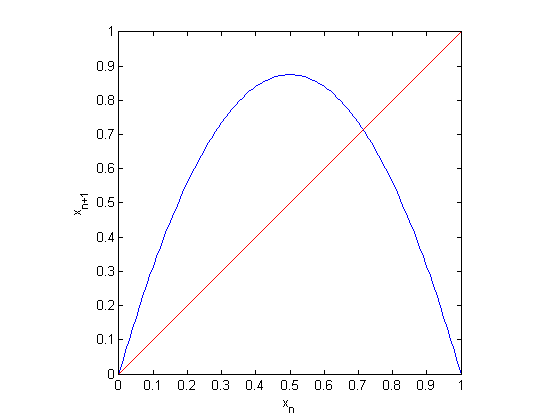
\includegraphics[scale=0.7]{deterministic}
\caption{The deterministic Logistic Map.}
	\end{center}
\end{figure}
\begin{figure}[H]
	\begin{center}
		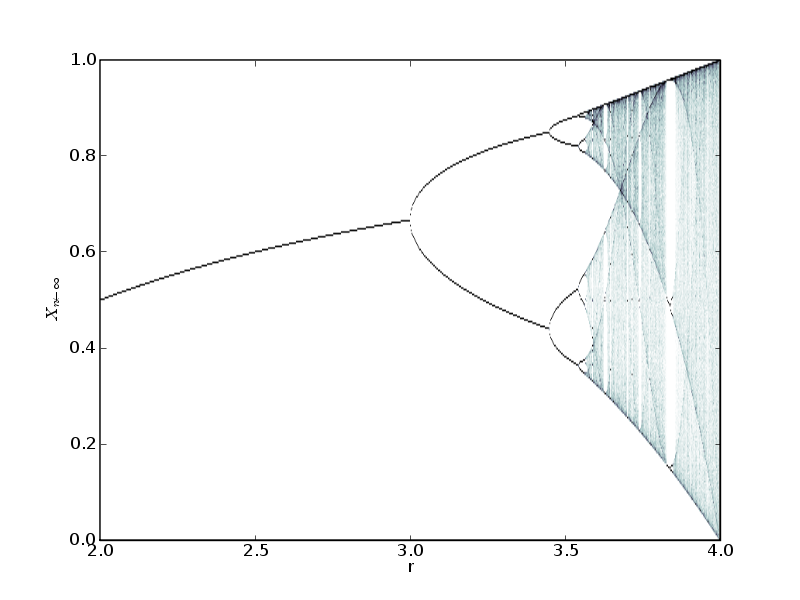
\includegraphics[scale=0.3]{det_bif}
\caption{The bifurcation diagram for the deterministic logistic
  map.}
	\end{center}
\end{figure}
Fixed points are located where the line $y=x$ intersects with the
Logistic Map. As the parameter $r$ is increased or decreased over the
interval [0,4], the map undergoes period doubling. Around $r=3.6$, the
map begins to display chaotic behavior.

\subsection{Random Logistic Map}
The Random Logistic function is a special case of the Logistic
function, which is not as popularly studied. In the random case, $r$ becomes a value dependent on $x$. Essentially, the Random Logistic
Map introduces the notion of spatial randomness to the deterministic
function (\ref{orig}). The Random Logistic function and map are as follows:
\begin{equation*}
f(x) = R(x)x(1-x)
\end{equation*}
\begin{equation}\label{randmap}
x_{n+1} = R(x_n)x_n(1-x_n)
\end{equation}
$R(x)$ consists of a Fourier series whose coefficients are independent
(but not identical) random variables drawn from a uniform
distribution whose bounds depend on the Fourier mode. 
\begin{align*}
\begin{split}
\ln(R(x)) &= \xi(x)\\
\xi(x) &= \ln(r) + 2\sum^N_{n=1}a_n\cos(2\pi nx)-b_n\sin(2\pi nx)\\
a_n,b_n &\sim Unif(-M_n,M_n)\\
M_n &= \sqrt{1.5S_n}\\
S_n &= \alpha e^{-L|n|}\\
\alpha &= \sigma^2 \tanh(L/2)\\
\sigma &< \ln(4/r)\frac{\tanh(L/4)}{\sqrt{1.5\tanh(L/2)}}
\end{split}
\end{align*}
Where $L \in (0,1)$ represents the correlation length (and is fixed
for each simulation) and $r \in [0,4]$ is also fixed for each simulation.

\begin{figure}[H]
	\begin{center}
		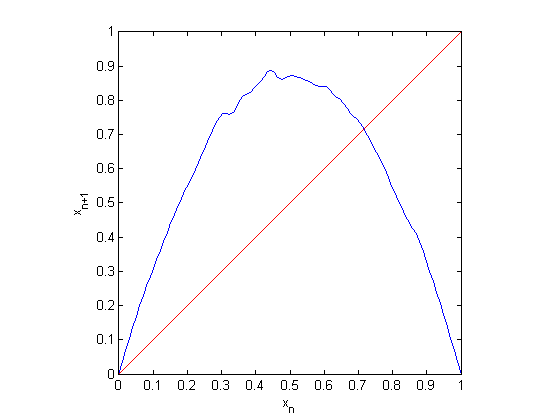
\includegraphics[scale=0.7]{random_cobweb}
\caption{One instance of a random logistic map. This is a preliminary result from the serial implementation.}
	\end{center}
\end{figure}
\begin{figure}[H]
	\begin{center}
		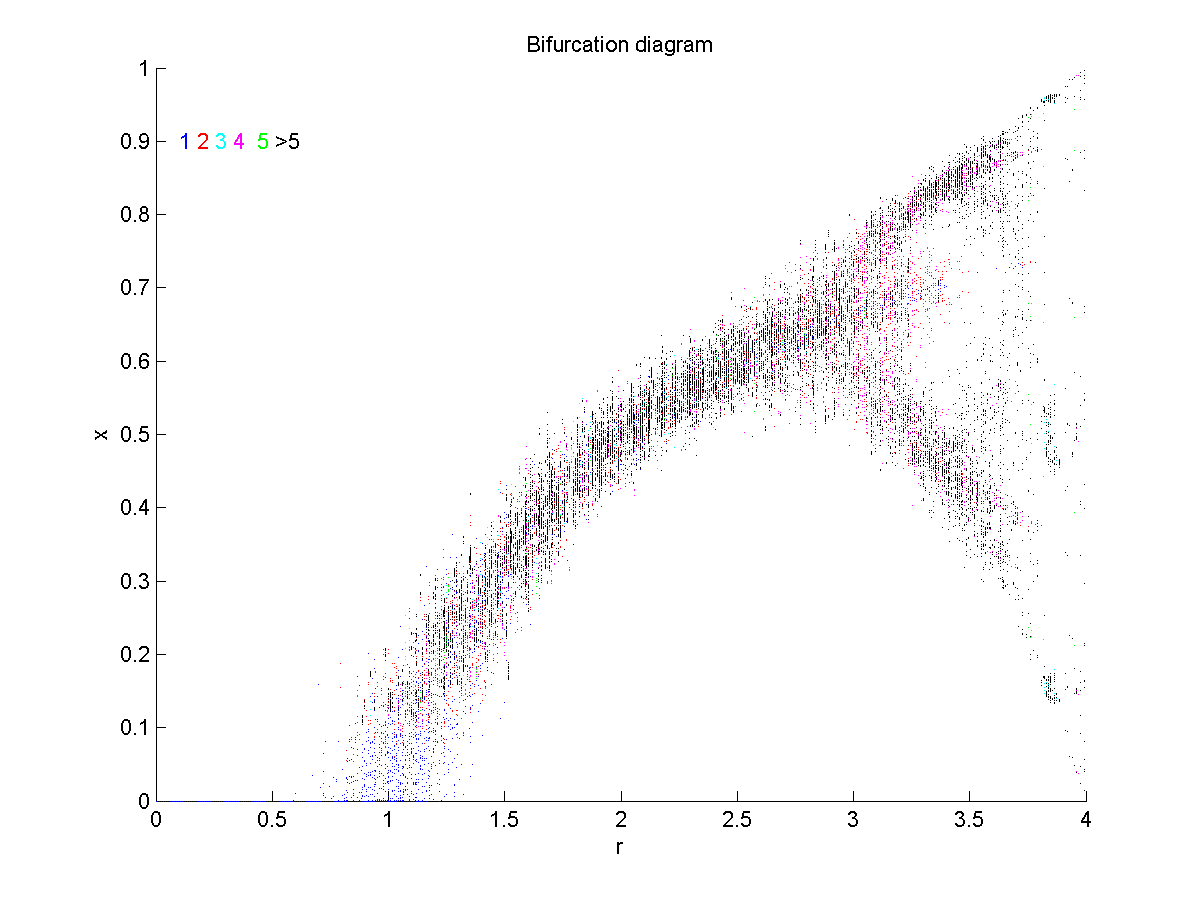
\includegraphics[scale=0.5]{bif}
\caption{The colors of the bifurcation diagram coincide with the
  period order in the legend (top left corner). This is a preliminary result from the serial implementation.}
	\end{center}
\end{figure}
An initial serial implementation has been developed for this project
and has been mildly tested in
MATLAB. Our project would consist of converting the existing code to
C++ and implementing parallelization through MPI with proper load balancing. Other possible improvements include
IO optimization and memory optimization (possible improvements through
HDF5). 

\subsection{Application to engineering}
This project has potential applications to civil engineering in terms
of treating contaminated groundwater \cite{neupauer}. Essentially, the
distribution of rocks underground can be viewed as a random field
distributed spatially, through which treatment solution must mix with
contaminated groundwater. Understanding the problem of spatial
randomness in one dimension can be generalized to two dimensions, with
the end goal of successfully simulating chaotic advection and reaction in two dimensions. 

\section{Analysis}
The analysis of our simulation will encompass the following:
\be
\item Compare the MFLOP/s (using profiling from psrun) for a variable number of simulation
sizes. 
\item Measure the speedup after implementing MPI. 
\item Analyze the Karp-Flatt Metric to see how the code
  performs in parallel. 
\item Compare the performance of our simulation in terms of GFLOP/s to
  the bite:flop ratio in the Roofline plot
\ee

\subsection{Testing}
Even though the nature of this project is random, it is possible to
compare the output of the parallel implementation to the serial
implementation for accuracy. The randomness lies in the function
$R(x)$, so using the same values of $R(x)$ for the serial and parallel
code should output the same results.


\bibliographystyle{plain}
\bibliography{proposal}

\end{document}
